\documentclass[a4paper,12pt]{article}

\usepackage{amsmath,amssymb,amsthm,tikz}
\usetikzlibrary{calc,arrows.meta}
\usepackage[margin=20mm]{geometry}
\usepackage{hyperref}

\setlength{\parindent}{0pt}
\setlength{\columnsep}{1cm}

\begin{document}

\twocolumn

\thispagestyle{empty}

\begin{center}
{\Large Assignment 14}\\
{\Large Published on 2020-12-06,}\\
{\em Estimated Time: 30 minutes,}\\
{\em Max.grade 10\textperthousand} 
\end{center}


\section{Bellman-Ford Algorithm}

The Bellman-Ford algorithm solves the single source shortest paths problem in
the case in which edge weights may be negative. It can work with directed graphs
(and also undirected graphs; not discussed in this exercise).  
The algorithm initializes the distances to all the vertices $u$ by $u.d = +\infty$. 
The only exception is the {\em source vertex}) which 
gets distance $s.d = 0$ (the distance to itself is $0$). 

After this initialization 
in a graph with $n$ vertices it will perform $n-1$ identical iterations. 
In every iteration it considers all the edges in some order, 
and ``relaxes'' all the edges. See (Goodrich2011, p.640), where
the edge relaxation procedure is described. 

After that the Bellman-Ford algorithm performs one last iteration: 
If there are still relaxations that reduce distances even after $n$ steps, 
this means that there is a negative loop in the original graph 
(and the shortest paths are not possible to compute as the distances can 
be reduced infinitely). 



\section{Problem}

Consider the graph in Figure~\ref{fig:problem-graph}.

\begin{figure}[!htb]
\center{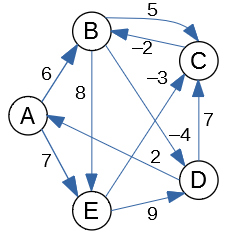
\includegraphics[width=2in]{assignment14-bellman-ford/problem-graph.png}}
\caption{\label{fig:problem-graph} Graph diagram}
\end{figure}

\vspace{10pt}
{\bf (A)} Find the following number: 
$$X = (a+b+c)\;\text{mod}\;5.$$
As a remainder it can take any value $0,1,2,3,4$. 
Depending on its value, select your source vertex 
from this table: 

\vspace{5pt}
\begin{tabular}{|c|c|c|c|c|c|} \hline
$X$ & $0$ & $1$ & $2$ & $3$ & $4$ \\ \hline
source & $A$ & $B$ & $C$ & $D$ & $E$  \\ \hline
\end{tabular}

\vspace{5pt}
Redraw the graph and mark your source vertex by a 
double-circle (or shade it, or draw a short incoming arrow 
or apply some other highlighting).

\vspace{10pt}
{\bf (B)} Create a table showing all the changes 
to all the distances to $A,B,C,D,E$ as the relaxations are performed. 
In a single iteration the same distance can be relaxed (improved) multiple times. 
In this case the table cell shows how the distance is changed in multiple steps
(e.g. $\infty \rightarrow 17 \rightarrow 11$).
The table should display all $n$ iterations (where $n=5$ is the number of vertices). 
The last iteration is not supposed to change/relax any distance (otherwise 
we have a negative loop).

{\em Note.} Please make sure to release the edges in the alphabetical/lexicographical order: 
Regardless of which is your source, in every iteration the edges are relaxed in this order: 
$$AB, AE, BD, BE, CB, DA, DC, EC, ED.$$
This would make your solution easier to verify.

\vspace{10pt}
{\bf (C)} Summarize the result: For each of the $5$ vertices 
tell what is its minimum distance from the source. 
Also tell what is the shortest path how to get there. 
For example, if your source is $E$ then you
could claim that the shortest path $E \leadsto B$ is 
of length $-5$ and it consists of two edges $(E,C)$, $(C,B)$. 






\end{document}

